% https://tex.stackexchange.com/a/765870/322482
\documentclass[tikz,border=5pt]{standalone}
\usepackage{newtxmath}
\usetikzlibrary{arrows.meta}
\begin{document}
    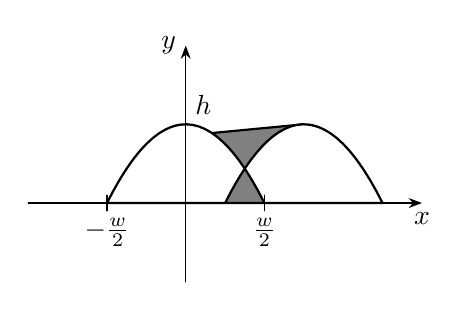
\begin{tikzpicture}[line cap=round,line join=round]
        % y=2/21*(x-1.5)+1
        \coordinate (tmp) at (0.75,{1-(0.75)^2});
        \draw[thick,fill=gray] (1/3,8/9) -- (1.5,1) -- (tmp) --cycle;
        \fill[white]
            plot[domain=-1:1] (\x, {1-(\x)^2}) -- cycle
            plot[domain=.5:2.5] (\x, {1-(\x-1.5)^2}) -- cycle;
        \begin{scope}[even odd rule]
            \draw[thick,fill=gray]
                plot[domain=-1:1] (\x, {1-(\x)^2}) -- cycle
                plot[domain=.5:2.5] (\x, {1-(\x-1.5)^2}) -- cycle
                plot[domain=-1:0.75] (\x, {1-(\x)^2}) -- (tmp) -- plot[domain=.75:2.5] (\x, {1-(\x-1.5)^2}) -- cycle
            ;
        \end{scope}
        \draw[-Stealth] (-2,0) -- (3,0) node[below] {$x$};
        \draw[-Stealth] (0,-1) -- (0,2) node[left] {$y$};
        \draw (-1,.1) -- ++(0,-.2) node[below=-1pt] {$-\frac{w}{2}$}
              (1,.1) -- ++(0,-.2) node[below=-1pt] {$\frac{w}{2}$}
              (0,1) node[above right] {$h$};
    \end{tikzpicture}
\end{document}